% File: tex/99_summary_SarazinFinoguenovWik_2012.tex
% Author: Timo L. R. Halbesma <timo.halbesma@student.uva.nl>
% Version: 0.01 (Initial)
% Date created: Mon Oct 26, 2015 04:16 PM
% Last modified: Tue Oct 27, 2015 03:53 PM
%
% Description: Literature Summary

% TODO: Lots of sentences have end weight due to changing order of things in sentece. This should be rewritten properly. 
\documentclass[MScProj_TLRH_ClusterEnergy.tex]{subfiles}
% Allow to compile this document on itself using the preamble of ../MScProj_TLRH_ClusterEnergy.tex

\usepackage{caption}
\usepackage{subcaption}

\begin{document}
\section*{Merger Shocks in Abell 3667 and the Cygnus A Cluster}
\label{sec:Sarazin2012}
Summary of \citet{2013AN....334..346S}.
\\
\textbf{Abstract}
XMM-Newton observations of the northwest radio relic region of Abell 3667 are presented, showing a jump in X-ray surface brightness and temperature which is indicative of a Mach 2 shock in that area. Combined with radio observations this yields an efficiency of 0.2 \% for dissipating shock kinetic energy into relativistic electron acceleration. Compared to Galactic supernova this efficiency is ten times lower but this can be explained by the lower Mach number. In addition, Suzaku observations of the Cygnus A radio galaxy are presented. The Cyg A radio source resides in an early-stage merging cluster of galaxies. The data show a hot region between the two sub-clusters in agreement with predictions of the shocked region. The radial velocity can be determined due to the high spectral resolution of Suzaku, and is found to be $\Delta v_r \approx 2650$ km/s.
\\

\textbf{Introduction}
Cluster mergers contribute to the formation of galaxy clusters at present time. Intracluster gas is thought to be heated primarily by energy injection due to cluster shocks. Cold fronts, merger bow shocks and other hydrodynamical phenomena are observed (see e.g. Markevitch \& Vikhlinin 2007). There are not a lot of observations of merger shocks.

\textbf{XMM-Newton Observations of a Shock at the NW Radio Relic in Abell 3667}
NB, The parts in chapter 2 about Abell 3667 are skipped.
A sharp surface brightness discontinuity implies a jump in gas density, see Eq.~\ref{eq:compression}, where 1 is pre-shock and 2 is post-shock. Here $C$ is the shock compression, and $n_e$ is the number density. Spectral observations showing a corresponding rise in gas temperature implies that a shock is seen. Using the Rankine-Hugoniot\footnote{I think, this is not given in the article} one finds the shock jump conditions Eq.~\ref{eq:shock_condition} and Eq.~\ref{eq:jump_condition}. NB, here $\gamma = 5/3$ such that the Mach number $\mathcal{M}$ can be calculated from the compression, or from the temperature ratio. Moreover, from Eq.~\ref{eq:shock_speed} the shock speed can be calculated.
% TODO: Derive shock conditions.

In addition, an order of magnitude estimate of the energy dissipated by the shock can be obtained starting with the change in kinetic energy flux given by Eq.~\ref{eq:KE_flux}, where $\rho_1$ it the pre-shock mass density in the gas.
% TODO: Derive energy flux equation.
The rate of conversion of shock kinetic energy is given by Eq.~\ref{eq:rate_of_conversion_energy}, where $A$ is the area of the shock perpendicular to the flow as a circle with a given radius.

\begin{align}
    C &= \frac{n_{e,2}}{n_{e,1}} \label{eq:compression} \\
    \frac{1}{C} &= \frac{3}{4 \mathcal{M}^2} + \frac{1}{4} \label{eq:shock_condition} \\
    \frac{T_2}{T_1} &= \frac{5 \mathcal{M}^4 + 14 \mathcal{M}^2 - 3}{16 \mathcal{M}^2} \label{eq:jump_condition} \\
    v_s &= \mathcal{M} c_{s1} \label{eq:shock_speed} \\
    \Delta F_{\rm KE} &= \frac{1}{2} \rho_1 v_s^3 \left( 1 - \frac{1}{C^2} \right ) \label{eq:KE_flux} \\
    \frac{dE_{\rm eE}}{dt} &= \Delta F_{\rm KE} A \label{eq:rate_of_conversion_energy} \\
    \epsilon &= \frac{\frac{dE_e}{dt}}{\frac{dE_{\rm KE}}{dt}} \approx \frac{L_{\rm NT}}{\frac{dE_{\rm KE}}{dt}} \approx 0.0021 \left[ \left( \frac{3.6 \mu G}{B} \right)^2 +1 \right] \label{eq:efficiency} \\
    t_{\rm rad} &\approx 1.3 \times 10^8 \left( \frac{\nu_b}{1.4 \text{ GHz}}\right)^{-1/2} \left( \frac{B}{3 \mu G} \right)^{-3/2} \times \left[ \left( \frac{3.6 \mu G}{B} \right)^2 +1 \right]^{-1} \text{ yr}  \label{eq:electron_age} \\
    \theta_{\rm rad} &= 1'.3 \left( \frac{\nu_b}{1.4 \text{ GHz}} \right)^{-1/2} \left( \frac{B}{3 \mu G} \right)^{-3/2} \times \left[ \left( \frac{3.6 \mu G}{B} \right)^2 +1 \right]^{-1} \cos \phi \label{eq:projected_distance}
\end{align}

% TODO: Derive efficiency equation.
It is possible to calculate the efficiency $\epsilon$ of heating the gas by assuming a steady state, setting the power required to (shock) accelerate electrons equal to the total luminosity, and assuming the luminosity is solely due to radiative energy loss of the relativistic electrons. See Eq.~\ref{eq:efficiency}, where $L_{\rm NT} \approx 3.8 10^{42} [(3.6 \mu G/B)^2] + 1$ erg s\Sup{-1} where $B$ is the magnetic field.
 
% TODO: Derive characteristic time equation.
Radiative losses cause a change in the spectrum because electrons are advected away from the shock. Specifically, a break at frequency $\nu_b$ can be observed from which the electron age can be inferred. See Eq.~\ref{eq:electron_age}

The projected distance of the electrons is given by Eq.~\ref{eq:projected_distance}. This is at the redshift of the cluster. $\phi$ is the angle between the central shock normal and the plane of the sky (?). Unrelated to this is the post-shock speed of material relative to the shock given by $v_2 = v_s/C$ km s\Sup{-1}.

First order Fermi acceleration is inconsistent with Abell 3667 as the expected power law spectrum $n(E) dE \propto E^{-p} dE$ for a power law index $p=(C+2)/(C-1)$, which in turn corresponds to a radio spectral index $\alpha = -(p-1)/2 \approx -1.55$. However, observations show a flatter spectrum with $\alpha \approx -0.7$, thus the shock compression is underestimated or the acceleration model is incorrect (not first order Fermi).

\textbf{Suzaku Measurement of the Merger Shock Velocity in the Cygnus A Cluster}
\begin{figure}
    \centering
    \begin{subfigure}[b]{0.4\textwidth}
        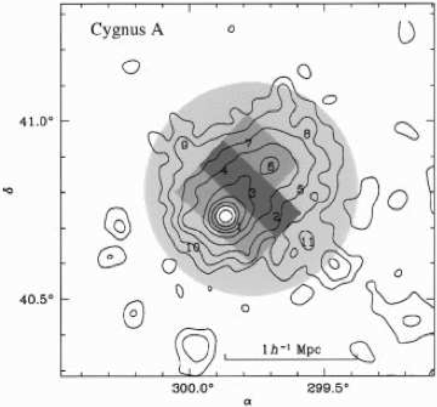
\includegraphics[width=\textwidth]{CygASuzaku3regions.png}
        \caption{ASCA X-ray grey-scale temperature map showing the three regions a spectrum was taken. Here lighter is lower temperature. The contours show a ROSAT image. From Markevitch, Sarazin, \& Vikhlinin (1999).}
        \label{fig:CygA_ASCA_3regions}
    \end{subfigure}
    ~ %add desired spacing between images, e. g. ~, \quad, \qquad, \hfill etc.       %(or a blank line to force the subfigure onto a new line)
    \begin{subfigure}[b]{0.4\textwidth}
        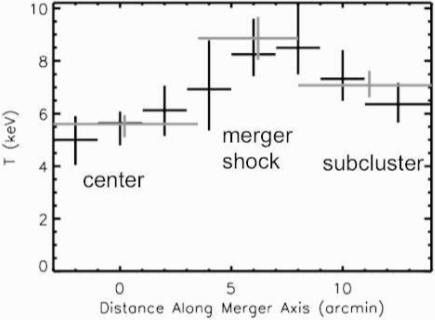
\includegraphics[width=\textwidth]{CygASuzaku3regionsTmap.png}
        \caption{Temperature vs distance along merger axis. Data from Suzaku. Here one can clearly see a higher temperature in the merger shock region as compared to the center and sub cluster regions. From \citet{2013AN....334..346S}.}
        \label{fig:CygA_Suzaku}
    \end{subfigure}
    \caption{Cygnus A images showing a higher temperature in the merger center.}\label{fig:CygA_SarazinFinoguenovWik2012}
\end{figure}

Einstein Observatory X-ray observations of Cygnus A have shown that the radio galaxy is surrounded by a moderately rich cluster, instead of lying in an isolated elliptical galaxy as was initially thought. Moreover, the cluster has a cool core of which the radio source Cygnus A is the center \citep{1984MNRAS.211..981A}. The Cygnus A cluster is undergoing a merger with a straightforward geometry, as can be seen in ASCA and Chandra observations \citep{1999ApJ...521..526M, 2002ApJ...565..195S}. Two sub clusters live inside the Cygnus A cluster of: one contains the Cygnus A radio source as central galaxy, and the other shows an excess in X-ray luminosity. See Fig.~\ref{fig:CygA_Suzaku}, where a higher temperature is visible in the merging region. The merger shock is reaonably symmetric and head-on. The merger is still at an early stage and the shocks have not yet reached the centers of the sub clusters.

Spectra show that the shock region is hotter than either sub cluster. This is expected because the gas between the sub clusters s shocked.

Fe K line gives the redshift. An increase is seen going from center to merger shock to sub cluster region.

One of the first direct detections of merger velocity using Doppler shifts of X-ray lines from intracluster gas.





\SubfileBibliography
\end{document}
